
\documentclass[10pt,a4paper]{article}
\usepackage[T1]{fontenc}
\usepackage{tikz}
\usepackage[margin=1cm]{geometry}
\begin{document}

\section*{Step-by-Step Binary Tree Construction:}
This document illustrates the step-by-step construction of a binary tree. Each step corresponds to the insertion of a new node, which modifies the tree structure as shown in the corresponding diagrams.

\subsection*{Explanation of Steps:}
The binary tree evolves with each insertion based on the user's input. Below, each step shows the state of the tree after a new node has been added. The nodes are placed according to the specified parent node and whether the new node is a left or right child.

\begin{figure}[h!]
\centering

\begin{minipage}{0.8\textwidth}
    \centering
    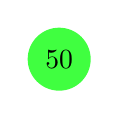
\begin{tikzpicture}[level distance=10mm]
        \tikzstyle{every node}=[fill=green!75,circle,inner sep=1pt, minimum size=8mm]
        \tikzstyle{level 1}=[sibling distance=30mm, set style={{every node}+=[fill=green!60]}]
        \tikzstyle{level 2}=[sibling distance=15mm, set style={{every node}+=[fill=green!45]}]
        \tikzstyle{level 3}=[sibling distance=10mm, set style={{every node}+=[fill=green!30]}]
        \tikzstyle{level 4}=[sibling distance=5mm, set style={{every node}+=[fill=green!15]}]
        \node {50} ;
    \end{tikzpicture}
    \caption{Step 1}
\end{minipage}
\vspace{1cm}

\begin{minipage}{0.8\textwidth}
    \centering
    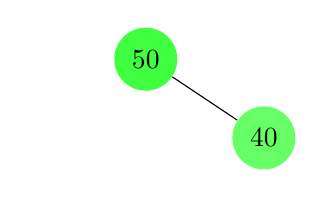
\begin{tikzpicture}[level distance=10mm]
        \tikzstyle{every node}=[fill=green!75,circle,inner sep=1pt, minimum size=8mm]
        \tikzstyle{level 1}=[sibling distance=30mm, set style={{every node}+=[fill=green!60]}]
        \tikzstyle{level 2}=[sibling distance=15mm, set style={{every node}+=[fill=green!45]}]
        \tikzstyle{level 3}=[sibling distance=10mm, set style={{every node}+=[fill=green!30]}]
        \tikzstyle{level 4}=[sibling distance=5mm, set style={{every node}+=[fill=green!15]}]
        \node {50} child[fill=none] {edge from parent[draw=none]} child {node {40} };
    \end{tikzpicture}
    \caption{Step 2}
\end{minipage}
\vspace{1cm}

\begin{minipage}{0.8\textwidth}
    \centering
    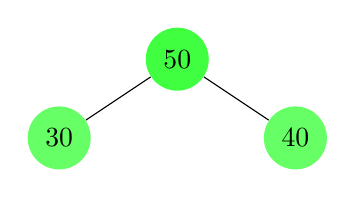
\begin{tikzpicture}[level distance=10mm]
        \tikzstyle{every node}=[fill=green!75,circle,inner sep=1pt, minimum size=8mm]
        \tikzstyle{level 1}=[sibling distance=30mm, set style={{every node}+=[fill=green!60]}]
        \tikzstyle{level 2}=[sibling distance=15mm, set style={{every node}+=[fill=green!45]}]
        \tikzstyle{level 3}=[sibling distance=10mm, set style={{every node}+=[fill=green!30]}]
        \tikzstyle{level 4}=[sibling distance=5mm, set style={{every node}+=[fill=green!15]}]
        \node {50} child {node {30} } child {node {40} };
    \end{tikzpicture}
    \caption{Step 3}
\end{minipage}
\vspace{1cm}

\begin{minipage}{0.8\textwidth}
    \centering
    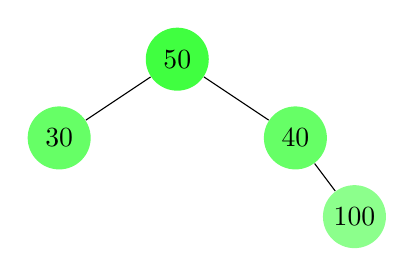
\begin{tikzpicture}[level distance=10mm]
        \tikzstyle{every node}=[fill=green!75,circle,inner sep=1pt, minimum size=8mm]
        \tikzstyle{level 1}=[sibling distance=30mm, set style={{every node}+=[fill=green!60]}]
        \tikzstyle{level 2}=[sibling distance=15mm, set style={{every node}+=[fill=green!45]}]
        \tikzstyle{level 3}=[sibling distance=10mm, set style={{every node}+=[fill=green!30]}]
        \tikzstyle{level 4}=[sibling distance=5mm, set style={{every node}+=[fill=green!15]}]
        \node {50} child {node {30} } child {node {40} child[fill=none] {edge from parent[draw=none]} child {node {100} }};
    \end{tikzpicture}
    \caption{Step 4}
\end{minipage}
\vspace{1cm}

\end{figure}
\newpage

\end{document}
